\documentclass{exam}
\usepackage{../../mypackages}
\usepackage{../../macros}

\setlength{\parindent}{0pt}

\title{Bac Blanc}
\author{N. Bancel}
\date{20 Novembre 2024}

\begin{document}

\textbf{Collège Lycée Suger}
\hfill
\textbf{Physique-Chimie} \\

\textbf{Année 2024-2025}
\hfill
\textbf{1ère STD2A} \par

{\let\newpage\relax\maketitle}


\begin{center}
  \textbf{\textcolor{blue}{Durée du devoir : 2 heures}} \par
  \vspace{1em}
  \textbf{\textcolor{red}{La calculatrice EST autorisée. Total des points : 21 points (1 point bonus)}} \par
  \vspace{1em}
\end{center}

\begin{tcolorbox}[colback=gray!10!white, colframe=gray, title=Note importante]
  \itshape{Toutes les réponses doivent être justifiées.
  La qualité et la précision de la rédaction seront prises en compte dans la notation des copies.
  Il est permis d'admettre le résultat de certaines questions pour ne pas rester bloqué, en prenant soin d'indiquer sur la copie les résultats admis. \par
  \vspace{1em}
  Exemples :
  \begin{itemize}
    \item Si vous connaissez par coeur le schéma de Lewis d'un atome mais n'êtes plus capable de le justifier, vous pouvez utiliser votre schéma appris par coeur pour résoudre les questions suivantes 
    \item Si une question demande d'avoir la réponse à la question précédente, vous pouvez expliquer comment vous auriez résolu le problème si vous aviez réussi la question précédente
  \end{itemize}
  }
\end{tcolorbox}

\section*{Exercice 1 [6 points] Questions de cours}

\subsection*{Les matériaux - 2 points}
\begin{questions}
  \question[1] Lister les 3 grandes familles de matériaux, et en donner une brève définition. Pour chaque famille, citer 2 exemples de matériaux.
  \question[0.5] Quelle est la différence entre un alliage et un métal pur ?
  \question[0.5] Définir un matériau composite et nommer ses 2 composants.

\end{questions}

\subsection*{L'atome - 1 point}

\begin{questions}
  \question[1] Pour l'atome d'oxygène (\ce{O}) de Numéro atomique : $Z = 8$ , donner : 

  \begin{itemize}[noitemsep]
    \item Sa configuration électronique (justifier comment on trouve le nombre d'électrons)
    \item Citer quelle est sa couche de valence, et son nombre d'électrons de valence 
    \item Dessiner son schéma de Lewis, en prenant bien soin de représenter les doublets non liants, et les électrons célibataires. 
  \end{itemize}
\end{questions}

\subsection*{Les polymères - 1 point}

\begin{questions}
\question[1] Donner la définition
\begin{parts}
  \part[0.25] D'un alcane
  \part[0.25] D'un alcène
  \part[0.5] D'un composé aromatique
\end{parts}
\end{questions}

\subsection*{Oxydoréduction - 2 points}

Ecrire les demi équations électroniques des couples Oxydant/Réducteur suivants
\begin{questions} 
  \question[0.5] \ce{Cu^{2+}/Cu}
  \question[0.75] \ce{I2/I^-}
  \question[0.75] \ce{H+/H2}
\end{questions}


\section*{Exercice 2 [7.5 points] Coulisses de Lascaux IV}

La grotte de Lascaux, découverte en 1940, a été fermée au grand public dès 1963 afin de préserver ses œuvres.  
Le Centre international d'art pariétal Lascaux IV, situé à Montignac, a été inauguré en décembre 2016.  
Il abrite un fac-similé de la grotte qui permet au grand public de redécouvrir ce trésor de l'art préhistorique.  

\subsection*{Le bâtiment et ses matériaux}

Lascaux IV est un bâtiment semi-enterré à la façade vitrée de longueur égale à 150 m.  
Il s'intègre parfaitement au paysage car l'arrière du bâtiment disparaît dans la forêt. \par
\vspace{1em}

Les architectes ont choisi de n'utiliser qu'un seul type de béton pour les sols, les parois, la toiture et la façade du bâtiment
afin de conférer à l'ensemble un aspect de grosse pierre et recréer au plus près la grotte d'origine.


\begin{tcolorbox}[colback=white, colframe=gray, coltitle=black, title=\textbf{Document 1 - Un chantier complexe}]
  Pour soutenir le bâtiment, dont la surface atteint $9000 m^2$, sur le sol peu stable et l'arrimer à la colline, il a fallu planter près de 550 pieux, certains jusqu'à la profondeur de 12 m.
  Près de 730 tonnes d'acier à béton ont été nécessaires. \\
  
  À l'intérieur du bâtiment, la réalisation de murs dont l'inclinaison peut atteindre la valeur de 9 degrés et dont la hauteur la plus importante prend la valeur de 12 m, reste une prouesse technique.
  Ils ont été coulés sur place avec un béton très fluide dans lequel ont été incorporés des gravillons.
  L'ensemble a dû ensuite être étayé de nombreux piliers. \\
  
  Ces grandes parois lisses penchées, avec des lignes horizontales paraissant gravées, rappellent aux visiteurs des roches sédimentaires qui plongent au centre de la Terre. \\

  L'autre défi technique a été la façade vitrée en forme de faille. Le vitrage, de longueur égale à 150 m, d'un seul tenant, est accroché par une structure métallique située en arrière.
  Le verre produit, avec le béton, une série d'effets de contraste : opacité/transparence ; pénombre/lumière ; brut/sophistiqué ; rugueux/lisse.
  \end{tcolorbox}

\begin{tcolorbox}[colback=white, colframe=gray, coltitle=black, title=\textbf{Document 2 - Des bétons}]
    Économique et facilement manipulable, le béton peut être utilisé dans divers domaines tels que la construction ou l'art. À la fois résistant et durable, il répond à de nombreux critères de performance, ce qui explique son omniprésence actuelle. […] \\

    Les principaux ingrédients employés pour le fabriquer sont le sable, le gravier, le ciment, le tout gâché avec de l'eau.  
    Le ciment est le liant hydraulique par excellence.  \\

    Le béton autoplaçant […] est un béton se différenciant des autres par son importante fluidité. […] Auparavant, il était fréquent de rajouter de l'eau au mélange afin d'obtenir un béton plus fluide mais cela le fragilisait. C'est pourquoi le béton autoplaçant est une véritable révolution. […] Si le béton autoplaçant possède une telle fluidité, c'est grâce aux divers adjuvants superplastifiants qu'il contient. Ceci a rendu les constructions plus sûres et a grandement facilité les méthodes de mise en œuvre du béton. […]. \\

    L'hyperfluidité facilite […] le remplissage des coffrages et l'enrobage des éventuelles armatures, tout en permettant de conserver une homogénéité. \\

    Le béton armé associe intimement un béton avec des armatures métalliques : on obtient ainsi un matériau qui cumule des qualités de résistance à la compression et à la traction.  
    Un enrobage soigné des armatures est toutefois nécessaire pour les préserver des phénomènes d'oxydation.
\end{tcolorbox}


\vspace{1em}
\textbf{Le béton - 3.5 points}

\begin{questions}
  \question[0.5] Le béton est omniprésent à Lascaux IV. Justifier le choix des architectes en citant une caractéristique esthétique et une caractéristique technique
  \question[0.5] Expliquer pourquoi le béton armé peut être considéré comme un matériau composite
  \question[0.5] Justifier la nécessité d'utiliser du béton autoplaçant pour réaliser les murs intérieurs du bâtiment.
  \question[1] Sachant que la masse volumique de l'acier est de \SI{7800}{kg/m^3}, et que $ \SI{1}{t} = \SI{1000}{kg}$, quel est le volume d'acier utilisé pour créer les pieux ?
  \question[1] On considère que cet acier a pu être acheminé dans des camions de \SI{25}{m^3}. Combien a-t-il fallu de camions pour transporter l'acier ? Et quel est le pourcentage de remplissage du dernier camion qui n'était pas rempli ?
\end{questions}

\vspace{1em}
\textbf{La structure métallique - 3 points}

\begin{questions}
  \question[0.5] En quelle matière est faite les pieux ?
  \question[2.5] Les espèces \ce{Fe} et \ce{Fe^{2+}} forment un couple oxydant-réducteur. Si le métal fer (\ce{Fe}) avait été choisi pour fabriquer les pieux, le phénomène de corrosion aurait pu être modélisé par une réaction d'oxydoréduction entre le métal fer et le dioxygène (\ce{O2}).
  \begin{parts}
    \part[0.5] Quelle est la demi équation électronique du couple oxydant/réducteur \ce{Fe^{2+}/Fe} ?
    \part[0.5] Le Fer (\ce{Fe}) est-il réduit ou oxydé ?
    \part[1] Compléter la demi-équation électronique du couple \ce{O2/HO^-} : \\
    \ce{O2 + ... H2O + ... e^- -> ... HO^-}
    \part[0.5] Le dioxygène (\ce{O2}) est-il réduit ou oxydé ?
  \end{parts}
\end{questions}

\vspace{1em}
\textbf{Le verre - 1 point}

\begin{questions}
  \question[0.5] A quelle catégorie de matériaux appartient le verre ? 
  \question[0.5] Quel est le principal composant du verre minéral ?
\end{questions}

\section*{Exercice 3 [7.5 points] The public collection}

\begin{tcolorbox}[colback=white, colframe=gray, coltitle=black, title=\textbf{Document 1 - Introduction}]
  The Public Collection, lancé en 2015 par l'artiste Rachel M. Simon et l'Indinia Public Library, est un projet de bibliothèques publiques miniatures en milieu urbain où chacun peut déposer ou récupérer des ouvrages gratuitement.
  Parmi les neuf propositions retenues figure \textit{Monument} du designer Brian McCutcheon, une structure à cinq piliers en aluminium supportant une citation de Marc Twain.
  À la base de chacune de ces colonnes se situe une étagère circulaire en polycarbonate où sont déposés les livres en libre accès.
\end{tcolorbox}

Le polycarbonate de la structure a été obtenu par réaction entre le phosgène et le Bisphénol A dont les formules topologiques sont données ci-dessous.

\begin{figure}[H]
  \centering
  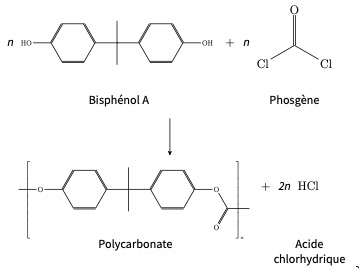
\includegraphics[width=0.8\linewidth]{01_02.jpg}
  \caption{Monument}
\end{figure} 

\begin{figure}[H]
  \centering
  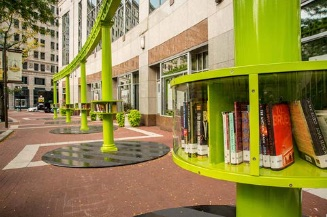
\includegraphics[width=0.4\linewidth]{01_03.jpg}
  \caption{Polymérisation}
\end{figure} 

\begin{questions}
  \question[0.5] À quelle famille appartient le Bisphénol A ? Justifier.
  \question[1] Repérer et nommer les groupes caractéristiques présents dans le Bisphénol A.
  \question[0.5] La fonction ester est-elle présente dans la molécule de polycarbonate ?
  \question[1] La réaction de synthèse du polycarbonate est-elle une polyaddition ou une polycondensation ?
  \question[1] Repérer et dessiner le motif élémentaire du polycarbonate.
  \question[1] Définir l'indice de polymérisation $n$
  \question[2.5] La structure aurait pu être faite à base de polypropylène (ou polypropène) isotactique, de sigle PP. C'est un polymère résistant, fabriqué à partir de molécules de Propylène par le réaction de polymérisation suivante : 
  
  \begin{figure}[H]
    \centering
    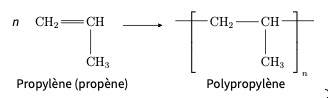
\includegraphics[width=0.8\linewidth]{01_04.jpg}
    \caption{Polymérisation}
  \end{figure} 
 
  
  \begin{parts}
  \part[1] Donner la formule développée du Propylène. Justifier
  \part[1] En déduire sa formule brute.
  \part[0.5] Est-ce un alcène ? Un alcane ? Un composé aromatique ? Justifier pourquoi.
  \end{parts}

\end{questions}

\end{document}
